\documentclass[a4paper]{article}

%% Language and font encodings
\usepackage[english]{babel}
\usepackage[utf8x]{inputenc}
\usepackage[T1]{fontenc}

%% Sets page size and margins
\usepackage[a4paper,top=3cm,bottom=2cm,left=2.7cm,right=2.7cm,marginparwidth=1.75cm]{geometry}

%% Useful packages
\usepackage{amsmath}
\usepackage{amsfonts}
\usepackage{bm}
\usepackage{graphicx}
\usepackage[colorinlistoftodos]{todonotes}
\usepackage[colorlinks=true, all colors=blue]{hyperref} %referenze linkate
\usepackage{booktabs}
\usepackage{siunitx}  %notaz. espon. con \num{} e unità di misura in SI con \si{}
\usepackage{xcolor}
\usepackage{colortbl}
\usepackage{bm}
\usepackage{caption} 
\usepackage{indentfirst}
\usepackage{physics} 
\usepackage{rotating}
\usepackage{tabularx}
\usepackage{url}
\usepackage{pst-plot}
\usepackage{comment} %per usare l'ambiente {comment}
\usepackage{float} 
\usepackage{subfig}
\usepackage[americanvoltages]{circuitikz} %per disegnare circuiti
\usepackage{tikz}
\usepackage{mathtools} %per allineare su più linee in ambiente {align} o {align*}
\usepackage{cancel}
\renewcommand{\CancelColor}{\color{lightgray}}
%\setlength{\parindent}{0cm}


\graphicspath{{Figure/}}
\captionsetup{format=hang,labelfont={sf,bf},font=small}
\captionsetup{tableposition=top,figureposition=bottom,font=small}
\captionsetup[table]{skip=8pt}

\newcommand{\meanv}[1]{\langle #1 \rangle}
\renewcommand{\hat}{\widehat}
\newcommand{\anto}{\hat{\psi}_{\lambda'}(\va{x}_1\tau_1)}
\newcommand{\basi}{ \hat{\psi}_{\mu'}(\va{x}_2\tau_2)}
\newcommand{\ciccio}{\hat{\psi}_\mu(\va{x}_2'\tau_2')}
\newcommand{\duccio}{\hat{\psi}_\lambda(\va{x}_1'\tau_1')}
\newcommand{\stanis}{\frac{e^{-\beta\hat{K}}}{Z_G}}
\newcommand{\lisa}{\lim_{\substack{\tau_1'\rightarrow\tau_1^+\\\tau_2'\rightarrow\tau_2^+}}}

\newcommand{\numberthis}{\addtocounter{equation}{1}\tag{\theequation}}



\newcommand{\Ta}{\Theta\pqty{\abs{\va{p}+\va{q}}-k_F}}
\newcommand{\Taa}{\Theta\pqty{k_F - \abs{\va{p}+\va{q}}}}

\newcommand{\Tb}{\Theta\pqty{\abs{\va{p} + \va{k} + \va{q}}-k_F}}
\newcommand{\Tbb}{\Theta\pqty{k_F - \abs{\va{p} + \va{k} + \va{q}}}}

\newcommand{\Tc}{\Theta\pqty{\abs{\va{p}+\va{k}}-k_F}}
\newcommand{\Tcc}{\Theta\pqty{k_F -\abs{\va{p}+\va{k}}}}

\newcommand{\Td}{\Theta\pqty{\abs{\va{p}}-k_F}}
\newcommand{\Tdd}{\Theta\pqty{k_F -\abs{\va{p}}}}

\newcommand{\Te}{\Theta\pqty{\abs{\va{p}-\va{k}}-k_F}}
\newcommand{\Tee}{\Theta\pqty{k_F -\abs{\va{p}-\va{k}}}}

\newcommand{\Tf}{\Theta\pqty{\abs{\va{k}}-k_F}}
\newcommand{\Tff}{\Theta\pqty{k_F -\abs{\va{k}}}}


\title{Domanda SubNuc}
\author{Giorgio Palermo}




\begin{document}
\hypersetup{linkcolor = black}
\hypersetup{linkcolor = blue}

\begin{center}
    \textbf{MASTER'S DEGREE IN PHYSICS}
    
    Academic Year 2019-2020
    
    \medskip
    \textbf{Introduction to Many Body Theory}
\end{center}

\vspace{0.8cm}
Student: Giorgio Palermo

Student ID: 1238258

Date: June 15, 2020

\bigskip

\begin{center}
\textbf{HOMEWORK 4}
\end{center}

\section*{Exercise 4.1}
As first step we show that the $(a), (c), (d), (e)$ contributions to the proper polarization (\ref{fig:first_order}) are vanishing.

\begin{figure}[h]
\centering
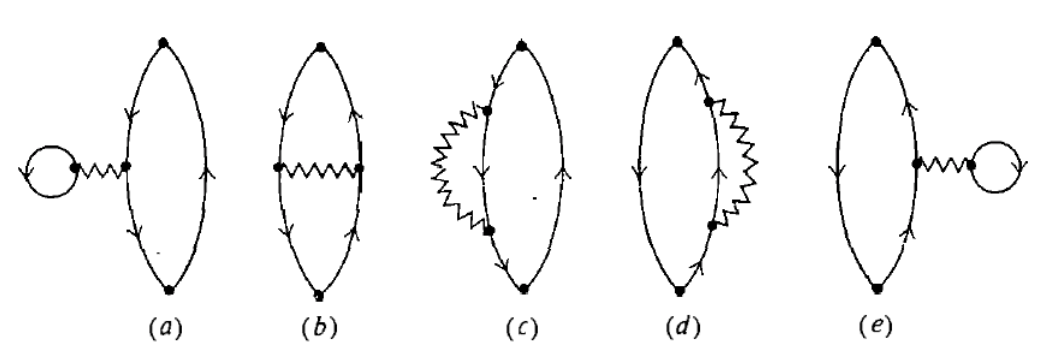
\includegraphics[width = .7\textwidth]{First_order.png}
\caption{All first-order contributions to proper polarization.}
\label{fig:first_order}
\end{figure}
The $(a)$ and $(e)$ contributions contain a $V(q=0)$ interaction term; in the special case of the degenerate electron gas these terms are precisely canceled by the action of the uniform positive background, as we shown in the lectures ([Fett-Wal] p. 154).

The $(c)$ contribution to the proper polarization can be written as:
\begin{equation}
\Pi^{*(c)} = -\frac{i}{(2\pi)^8}\pqty{\frac{1}{\hbar}}^2\int \dd[4]{p}\dd[4]{k}G^0(p+q)G^0(p)U^0(k)G^0(p-k)G^0(p)
\end{equation}
\begin{figure}[t]
\centering
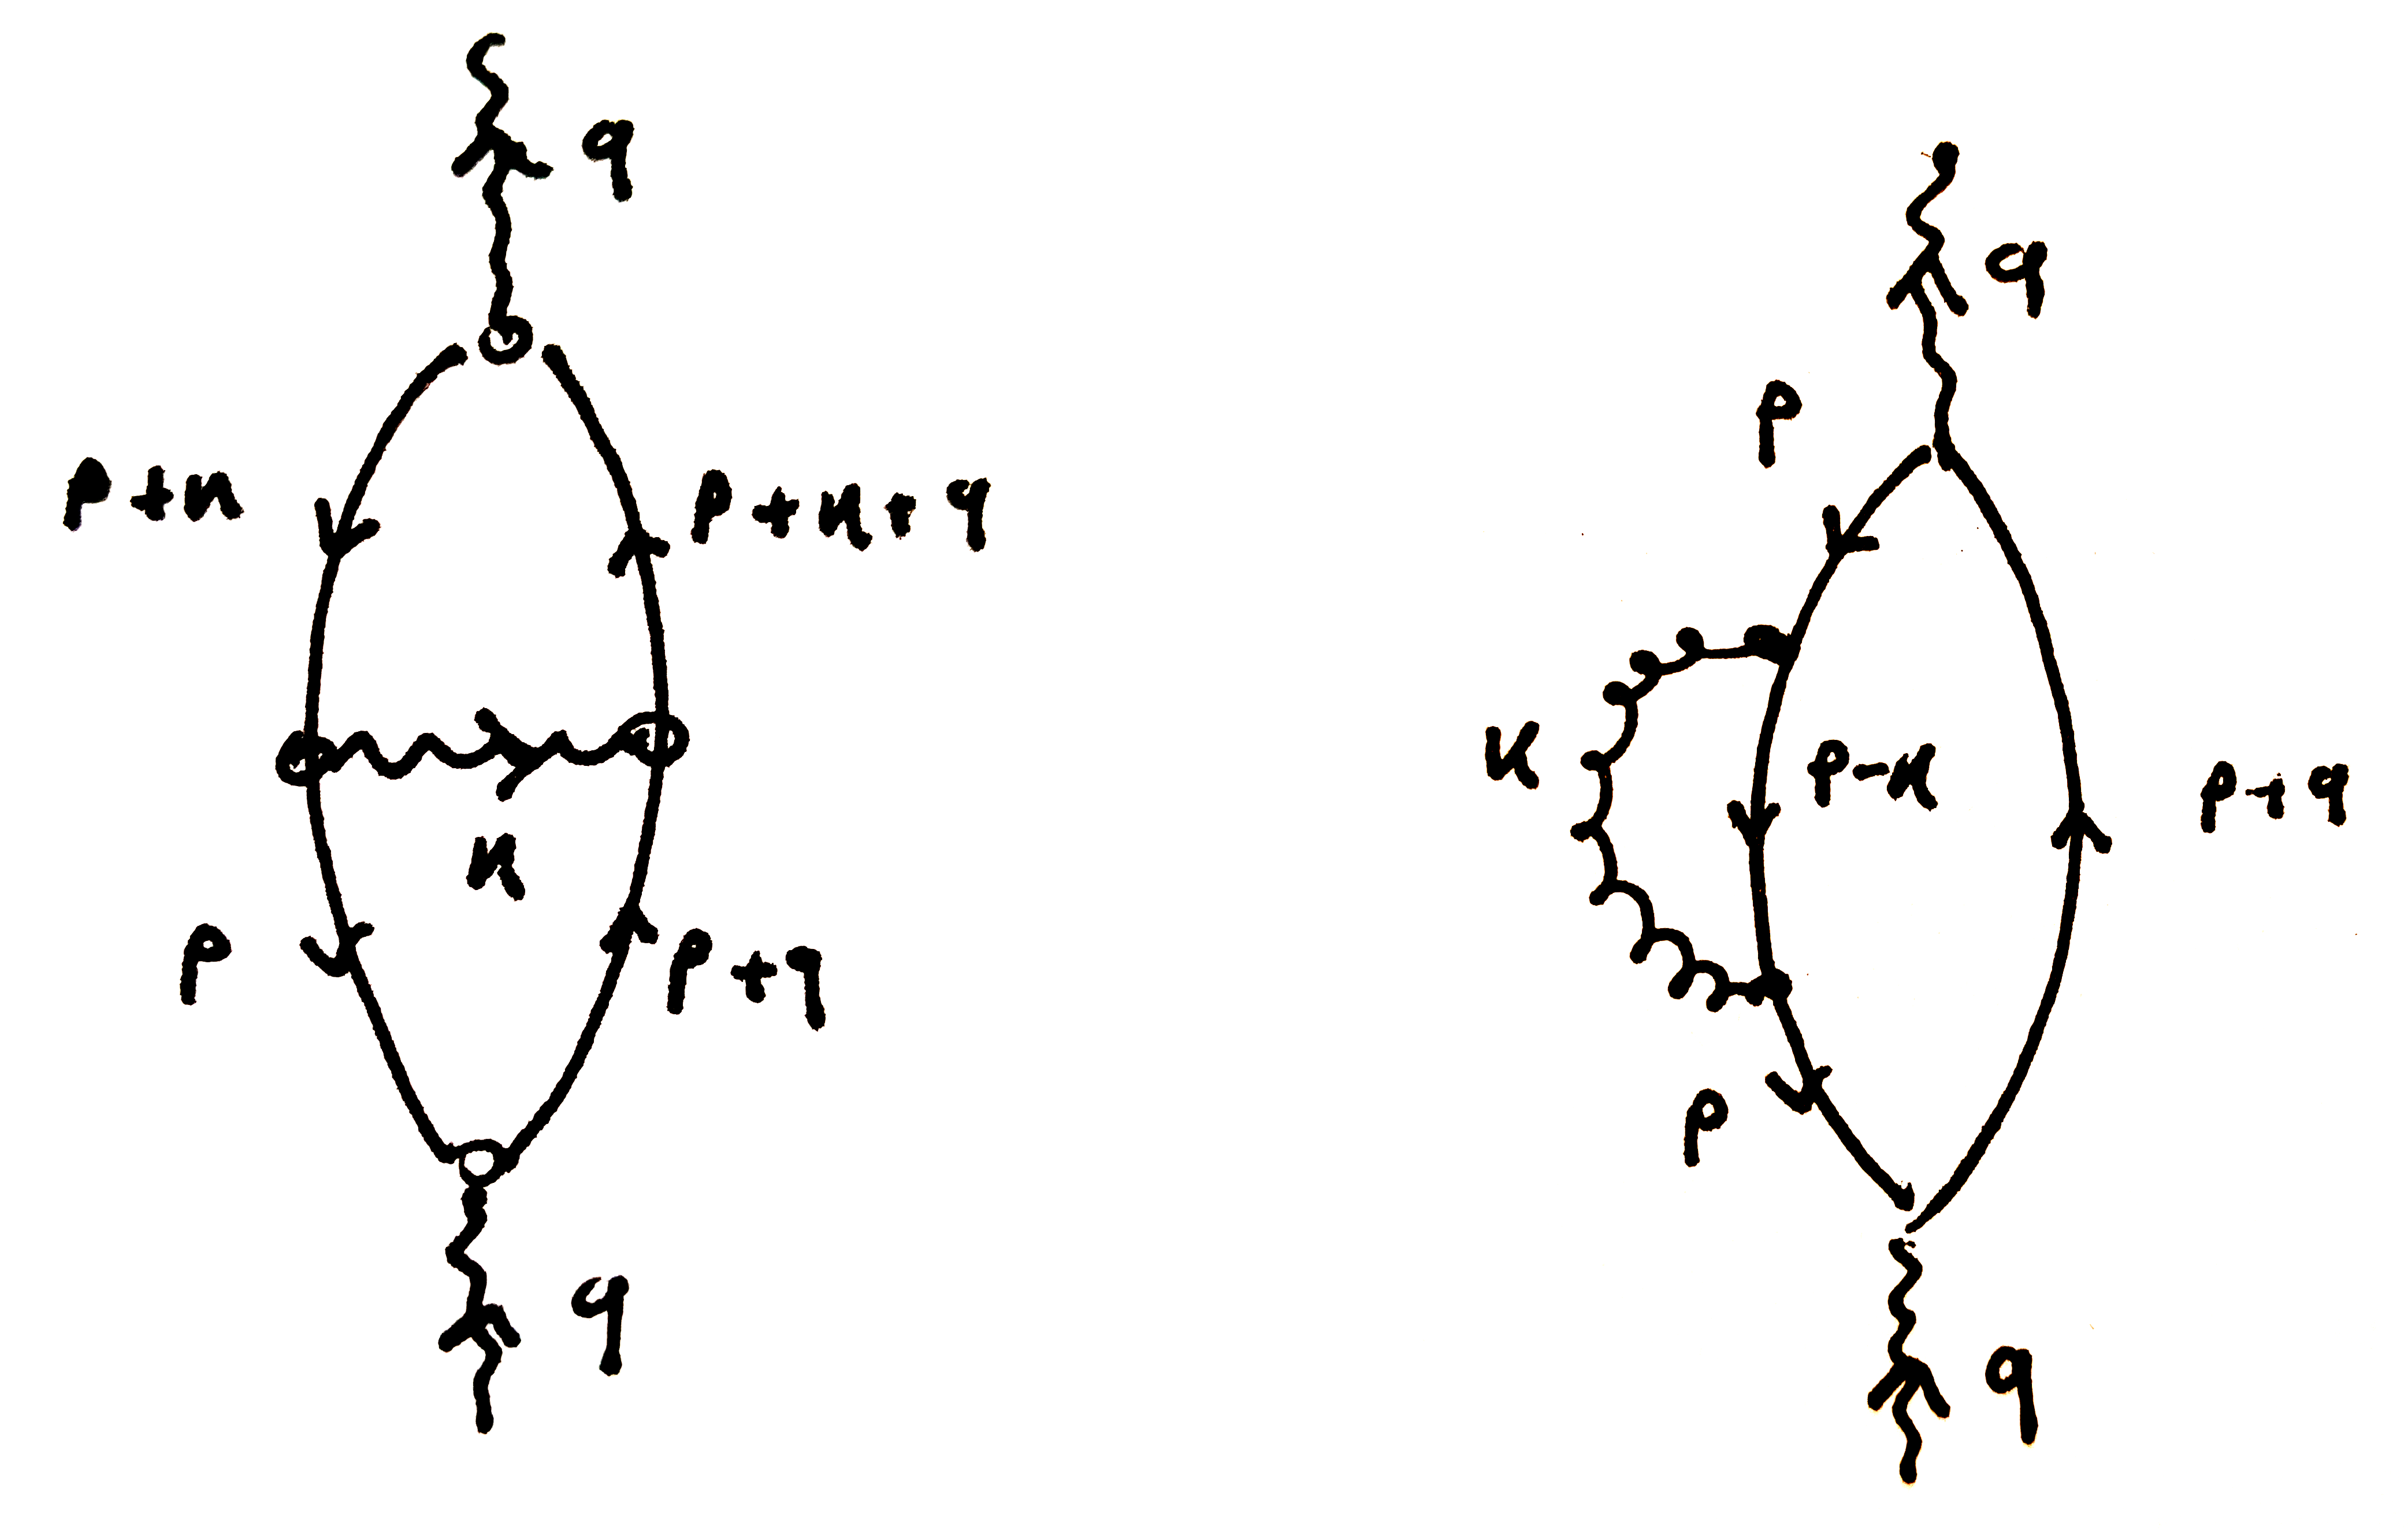
\includegraphics[width=.55\textwidth]{b_c_diagram.png}
\caption{$(b)$ and $(c)$ contributions to proper polarization.}
\label{fig:b_diagram}
\end{figure}
which leads to the energy contribution:
\begin{align*}
E_2^{(c)} \propto \int \dd[4]{q}\dd[4]{p}\dd[4]{k}&V_0(\va{q}) V_0(\va{p} -\va{k})
\bqty{\frac{\Td}{p^0-\omega_{\va{p}} +i\eta}+ \frac{\Tdd}{p^0+\omega_{\va{p}} -i\eta}}^2 \times \\
&\times\bqty{\frac{\Ta}{p^0 +q^0 -\omega_{\va{p} + \va{q}} + i\eta} + \frac{\Taa}{p^0+q^0 -\omega_{\va{p}+\va{q}}-i\eta}}\times\\
&\times \bqty{\frac{\Tf}{k^0-\omega_{\va{k}} +i\eta}+ \frac{\Tff}{k^0+\omega_{\va{k}} -i\eta}},\numberthis \\\label{eq:c_con}
\end{align*}
where in the last expression we substituted the expression for the bare Green function and we let the numerical factors apart.
Now, focusing on the integration over $p^0,$ we see that a simplification occur over the terms deriving from $G^0(p)G^0(p):$ the terms formed with $\Td\Tdd$ vanish, because the product of the two Heaviside step functions is non null only over the $\abs{\va{p}} = k_F$ point.
Since the square of a step function is a step function itself, the expression is then:
\begin{align*}
E_2^{(c)} \propto \int \dd[3]{\va{p}}\dd{p^0}&
\bqty{\frac{\Td}{\pqty{p^0-\omega_{\va{p}} +i\eta}^2}+ \frac{\Tdd}{\pqty{p^0+\omega_{\va{p}} -i\eta}^2}} \times \\
&\times\bqty{\frac{\Ta}{p^0 +q^0 -\omega_{\va{p} + \va{q}} + i\eta} + \frac{\Taa}{p^0+q^0 -\omega_{\va{p}+\va{q}}-i\eta}}\times.\numberthis\\
\end{align*}
All the products formed by factors with the complex part $\pm i\eta$ on the same side of the real axis vanish, because, using the residue theorem, we can close the integration path over a region with no poles and therefore null residue; we remain only with:
\begin{align*}
\Pi^{*(c)} \propto \int \dd[3]{\va{p}}\dd{p^0}&
\bqty{\frac{\Td\Taa}{\pqty{p^0-\omega_{\va{p}} +i\eta}^2\pqty{p^0+q^0 -\omega_{\va{p}+\va{q}}-i\eta}}+ \frac{\Tdd\Ta}{\pqty{p^0+\omega_{\va{p}} -i\eta}^2\pqty{p^0 +q^0 -\omega_{\va{p} + \va{q}} + i\eta}}} .\numberthis \\
\end{align*}
which is equal, using the residue theorem, to:
\begin{align*}
= 2\pi i\bqty{\frac{\Td\Taa}{\pqty{-q^0 +\omega_{\va{p}+\va{q}}-\omega_{\va{p}}+i\eta}^2}- \frac{\Tdd\Ta}{\pqty{-q^0 +\omega_{\va{p}+\va{q}}-\omega_{\va{p}}-i\eta}^2}} .\numberthis \\
\end{align*}
Now, substituting back into the expression for the energy:
\begin{align*}
E_2^{(c)} \propto\int \dd[3]{\va{q}}\dd{q^0}\dd[3]{\va{p}}\dd[4]{k}& V_0(\va{p} -\va{k})
\bqty{\frac{\Td\Taa}{\pqty{-q^0 +\omega_{\va{p}+\va{q}}-\omega_{\va{p}}+i\eta}^2}- \frac{\Tdd\Ta}{\pqty{-q^0 +\omega_{\va{p}+\va{q}}-\omega_{\va{p}}-i\eta}^2}} \times \\
&\times \bqty{\frac{\Tf}{k^0-\omega_{\va{k}} +i\eta}+ \frac{\Tff}{k^0+\omega_{\va{k}} -i\eta}}.\numberthis \\
\end{align*}
However, integrating over $q^0$ we find a pole of order two and, since the numerator is constant with respect to $q^0,$ the result of the integral is vanishing, and also the energy contribution.
The same procedure can be used to prove that the $(c)$ energy contribution vanishes as well.








\bigskip




The next step is the evaluation of the $(b)$ term in figure \ref{fig:first_order} with the aim of computing the $(b)$ first order contribution to the correlation energy $E_2^(b).$
In figure \ref{fig:b_diagram} the diagram is written in momentum space with the momentum conserved at each node; the spin part is omitted since it's easily proven that its contraction gives a $2s+1 \overset{s=1/2}{\rightarrow} 2 $ factor; this is due to the fact that each non interacting GF is diagonal in spin space and the interaction is spin-independent.
The analytic expression associated to the diagram in \eqref{fig:b_diagram} is:
\begin{align*}
\Pi^{*(b)}_2 = -\frac{2}{(2\pi)^8}\pqty{\frac{i}{\hbar}}^2\int\dd[4]{k}\dd[4]{p}G^0\pqty{\va{p}+\va{q}}G^0\pqty{\va{p}+\va{k}+\va{q}}G^0\pqty{\va{p}+\va{k}}U^0\pqty{\va{k}}G^0\pqty{\va{p}}
\end{align*}
that can be written explicitly knowing the expression of the GF for free fermions in momentum space as:
\begin{align*}
\int \frac{\dd[4]{q}}{(2\pi)^4}U^0(q)\Pi^*(q) = -\frac{2(4\pi e)^2}{(2\pi)^{12}} \pqty{\frac{i}{\hbar}}^2 &\int \dd[4]{q}\dd[4]{p}\dd[4]{k}\frac{1}{\va{q}^2 \va{k}^2}
\bqty{\frac{\Ta}{p^0 +q^0 -\omega_{\va{p} + \va{q}} + i\eta} + \frac{\Taa}{p^0+q^0 -\omega_{\va{p}+\va{q}}-i\eta}}\times\\
&\times \bqty{\frac{\Tb}{p^0+q^0+k^0 - \omega_{\va{p}+\va{k}+\va{q}}+i\eta} + \frac{\Tbb}{p^0+q^0+k^0 - \omega_{\va{p}+\va{k}+\va{q}}-i\eta} }\times\\
&\times \bqty{\frac{\Tc}{p^0+k^0 - \omega_{\va{p}+\va{k}}+i\eta} + \frac{\Tcc}{p^0+k^0 - \omega_{\va{p}+\va{k}}-i\eta} }\times\\
&\times \bqty{\frac{\Td}{p^0 - \omega_{\va{p}}+i\eta} + \frac{\Tdd}{p^0 - \omega_{\va{p}}-i\eta} }.\numberthis 
\end{align*}
where in the last expression we added the integration over $q$ and a $U^0(q)$ factor to make the expression closer to the one we need for the computation of the energy.
The evaluation of this integral starts from the temporal component $k^0$ relative to the four-vector $k;$ observing the expression we note that some of the products involved in the $k^0$ integration present both poles on the same side (above or below) of the $k^0$ complex plane; this means that, for these terms, the integration over the real variable $k^0$ can be extended to an integration on the complex plane that does not include any pole and is therefore vanishing.
For this reason we can rearrange the previous expression keeping only the non vanishing terms:
\begin{align*}
= -\frac{2(4\pi e)^2}{(2\pi)^{12}} \pqty{\frac{i}{\hbar}}^2 \int \dd[4]{q}\dd[4]{p}\dd[3]{\va{k}}\dd{k^0}&\frac{1}{\va{q}^2 \va{k}^2}
\bqty{\frac{\Ta}{p^0 +q^0 -\omega_{\va{p} + \va{q}} + i\eta} + \frac{\Taa}{p^0+q^0 -\omega_{\va{p}+\va{q}}-i\eta}}\times\\
&\times \bqty{\frac{\Td}{p^0 - \omega_{\va{p}}+i\eta} + \frac{\Tdd}{p^0 - \omega_{\va{p}}-i\eta} }\times\\
&\times \left[\frac{\Tcc\Tb}{\pqty{p^0+k^0 - \omega_{\va{p}+\va{k}}-i\eta}\pqty{p^0+q^0+k^0 - \omega_{\va{p}+\va{k}+\va{q}}+i\eta}} \right.+\\
&+\left. \frac{\Tc\Tbb}{\pqty{p^0+k^0 - \omega_{\va{p}+\va{k}}+i\eta}\pqty{p^0+q^0+k^0 - \omega_{\va{p}+\va{k}+\va{q}}-i\eta}}\right]\numberthis .
\end{align*}
The integral over $k^0$ can be evaluated using the residues theorem computing the residues at $\bar{q}^0_a = p^0 +\omega_{\va{p}+\va{k}} +i\eta$ for the first term and at $\bar{q}^0_b = p^0 +\omega_{\va{p}+\va{k}} -i\eta$ for the second one, obtaining:
\begin{align*}
= -\frac{2(4\pi e)^2}{(2\pi)^{12}} \pqty{\frac{i}{\hbar}}^2 \int \dd[4]{q}\dd[4]{p}\dd[3]{\va{k}}&\frac{1}{\va{q}^2 \va{k}^2}
\bqty{\frac{\Ta}{p^0 +q^0 -\omega_{\va{p} + \va{q}} + i\eta} + \frac{\Taa}{p^0+q^0 -\omega_{\va{p}+\va{q}}-i\eta}}\times\\
&\times \bqty{\frac{\Td}{p^0 - \omega_{\va{p}}+i\eta} + \frac{\Tdd}{p^0 - \omega_{\va{p}}-i\eta} }\times\\
&\times \left[\frac{\Tcc\Tb}{p^0+q^0+ \omega_{\va{p}+\va{k}}- \omega_{\va{p}+\va{k}+\va{q}}+i\eta} \right.-\\
&-\left. \frac{\Tc\Tbb}{p^0+q^0+ \omega_{\va{p}+\va{k}}- \omega_{\va{p}+\va{k}+\va{q}}-i\eta}\right]\numberthis .
\end{align*}
An analogous procedure helps us to compute the integration over the $p^0$ temporal component; in this case the expression to evaluate reduces to:
\begin{align*}
= -\frac{2(4\pi e)^2}{(2\pi)^{12}} \pqty{\frac{i}{\hbar}}^2 \int \dd[4]{q}\dd[3]{\va{p}}\dd{p^0}\dd[3]{\va{k}}&\frac{1}{\va{q}^2 \va{k}^2}
\left[\frac{\Ta\Tdd}{\pqty{p^0 +q^0 -\omega_{\va{p} + \va{q}} + i\eta}\pqty{ p^0 - \omega_{\va{p}}-i\eta}}\right.\\
& + \left.\frac{\Taa\Td}{\pqty{p^0 +q^0 -\omega_{\va{p} + \va{q}} - i\eta}\pqty{ p^0 - \omega_{\va{p}}+i\eta}}\right]\times\\
&\times \left[\frac{\Tcc\Tb}{p^0+q^0+ \omega_{\va{p}+\va{k}}- \omega_{\va{p}+\va{k}+\va{q}}+i\eta} \right.+\\
&+\left. \frac{\Tc\Tbb}{p^0+q^0+ \omega_{\va{p}+\va{k}}- \omega_{\va{p}+\va{k}+\va{q}}-i\eta}\right]\numberthis,
\end{align*}
and the poles to compute the residues are located respectively at $p^0_a = \omega_{\va{p}} + i\eta$ and at $p^0_b = \omega_{\va{p}} - i\eta.$
The result is the following:
\begin{align*}
 = -\frac{2(4\pi e)^2}{(2\pi)^{12}} \pqty{\frac{i}{\hbar}}^2 \int \dd[4]{q}\dd[3]{\va{p}}\dd{p^0}\dd[3]{\va{k}}&\frac{1}{\va{q}^2 \va{k}^2}
\left[\frac{\Ta\Tdd}{q^0 +\omega_{\va{p}}-\omega_{\va{p} + \va{q}} + i\eta}\right.\\
& - \left.\frac{\Taa\Td}{q^0 +\omega_{\va{p}}-\omega_{\va{p} + \va{q}} - i\eta}\right]\times\\
&\times \left[\frac{\Tcc\Tb}{p^0+q^0+ \omega_{\va{p}+\va{k}}- \omega_{\va{p}+\va{k}+\va{q}}+i\eta} \right.+\\
&+\left. \frac{\Tc\Tbb}{p^0+q^0+ \omega_{\va{p}+\va{k}}- \omega_{\va{p}+\va{k}+\va{q}}-i\eta}\right]\numberthis .
\end{align*}
The last integration is over the $q^0$ temporal part; keeping again the non vanishing terms we get:
\begin{align*}
 = +\frac{2(4\pi e)^2}{(2\pi)^{12}} \pqty{\frac{i}{\hbar}}^2 \int \dd[3]{\va{q}}\dd[3]{q^0}\dd[3]{\va{p}}\dd[3]{\va{k}}&\frac{1}{\va{q}^2 \va{k}^2}
\left[\frac{\Ta\Tdd\Tc\Tbb}{\pqty{q^0 +\omega_{\va{p}}-\omega_{\va{p} + \va{q}} + i\eta}\pqty{p^0+q^0+ \omega_{\va{p}+\va{k}}- \omega_{\va{p}+\va{k}+\va{q}}-i\eta}}\right.\\
& + \left.\frac{\Taa\Td\Tcc\Tb}{\pqty{q^0 +\omega_{\va{p}}-\omega_{\va{p} + \va{q}} - i\eta}\pqty{{p^0+q^0+ \omega_{\va{p}+\va{k}}- \omega_{\va{p}+\va{k}+\va{q}}+i\eta}}}\right]\numberthis.
\end{align*}
and the concerned poles are $q^0_a = \omega_{\va{p}+\va{q}} -\omega_{\va{p}} -i \eta $ and $q^0_b = \omega_{\va{p}+\va{q}} -\omega_{\va{p}} +i \eta:$
\begin{align*}
= +\frac{2(4\pi e)^2}{(2\pi)^{12}} \pqty{\frac{i}{\hbar}}^2 \int \dd[3]{\va{q}}\dd[3]{\va{p}}\dd[3]{\va{k}}&\frac{1}{\va{q}^2 \va{k}^2}
\left[\frac{\Ta\Tdd\Tc\Tbb}{\omega_{\va{p}} -\omega_{\va{p}-\va{q}} +\omega_{\va{p}+\va{k}} - \omega_{\va{p}+\va{k}+ \va{q}}}\right.\\
& + \left.\frac{\Taa\Td\Tcc\Tb}{\omega_{\va{p}} -\omega_{\va{p}-\va{q}} +\omega_{\va{p}+\va{k}} - \omega_{\va{p}+\va{k}+ \va{q}}}\right]\numberthis.
\end{align*}
Note that in the last step we removed the complex $i\eta$ terms since the temporal part has been completely evaluated.
Now we proceed with a change of variables in order to exploit the symmetry of the expression and simplify one of the addends; the change
\begin{equation}
\begin{cases}
\va{p}\rightarrow-\va{p} -\va{q}\\
\va{k} \rightarrow -\va{k}
\end{cases}
\end{equation}
applied to the second addend modifies the numerator to:
\begin{equation}
\Ta\Tdd\Tc\Tbb
\end{equation}
which allows us to write the integral in a more compact form as:
\begin{align}
= +\frac{4(4\pi e)^2}{(2\pi)^{12}} \pqty{\frac{i}{\hbar}}^2 \int \dd[3]{\va{q}}\dd[3]{\va{p}}\dd[3]{\va{k}}&\frac{1}{\va{q}^2 \va{k}^2}
\left[\frac{\Ta\Tdd\Tc\Tbb}{\omega_{\va{p}} -\omega_{\va{p}-\va{q}} +\omega_{\va{p}+\va{k}} - \omega_{\va{p}+\va{k}+ \va{q}}}\right]
\end{align}
On the other hand, the denominator can also be written more explicitly as:
\begin{align}
\omega_{\va{p}} -\omega_{\va{p}-\va{q}} +\omega_{\va{p}+\va{k}} - \omega_{\va{p}+\va{k}+ \va{q}}
=-\frac{\hbar}{2m} \bqty{\va{q}^2 - \va{q}\vdot\pqty{\va{p}+\va{k}}}
\end{align}
A scaling of the variables by a $k_F^{-1}$ factor brings in front an overall $k_F^3$ factor; simplifying some elements one gets:
\begin{align}
= -\frac{2ie^4mk_F^3}{\pi^3\hbar^3}\int \dd[3]{\va{q}}\dd[3]{\va{p}}\dd[3]{\va{k}}
\left[\frac{\Ta\Tdd\Tc\Tbb}{(\va{p}+\va{q}+\va{k})^2\bqty{\va{q}^2 - \va{q}\vdot\pqty{\va{p}+\va{k}}}}\right]
\end{align}
The second order $(b)$ energy contribution differs from the expression we computed for a $i\hbar V /2/(2\pi)^4$ factor; using the expression for the Fermi moment $k_F^3 = 3\pi^2N/V$ we get:
\begin{align*}
-\frac{2ie^4mk_F^3}{\pi^3\hbar^3} \frac{i\hbar V}{2(2\pi)^4} 3\pi^2\frac{N}{V} = \frac{3}{16\pi^5}\frac{e^4mN}{\hbar^2} = \frac{3}{16\pi^5} \frac{e^2N}{a_0}
\end{align*}
where $a_0 = \hbar^2/(me^2)$ is the Bohr radius.
The final expression for the second order contribution to the correlation energy is therefore
\begin{align}
E_2^{(b)} = \frac{3}{16\pi^5}\pqty{\frac{e^2N}{a_0}}\int\frac{\dd[3]{\va{q}}}{\va{q}^2}\int_{\abs{\va{k}+\va{q}}>1}\dd[3]{\va{k}}\int_{\abs{\va{p}+\va{q}}>1}\dd[3]{\va{p}}\frac{\Theta\pqty{1-\abs{\va{k}}}\Theta\pqty{1-\abs{\va{p}}}}{(\va{p}+\va{q}+\va{k})^2\bqty{\va{q}^2 - \va{q}\vdot\pqty{\va{p}+\va{k}}}}
\end{align}
as we wanted to prove.


















\section*{Exercise 7.1}
For a generic one particle operator $\hat{O}$ the grand canonical ensemble average is defined as
\begin{equation}
\meanv{\hat{O}} = \Tr{\hat{\rho}_G \hat{O}} = \int \dd[3]{\va{x}} \lim_{\va{x}'\rightarrow\va{x}}\Tr{\widehat{\rho}_{G} \hat{\psi}_{\alpha}^{\dagger}\left(\va{x}^{\prime}\right) O_{\alpha \beta}(\va{x}) \hat{\psi}_{\beta}(\va{x})}
= \int \dd[3]{\va{x}} \lim_{\va{x}'\rightarrow\va{x}} O_{\alpha\beta}\Tr{\frac{e^{-\beta\hat{K}}}{Z_G}\hat{\psi}_{\alpha}^{\dagger}\left(\va{x}^{\prime}\right)  \hat{\psi}_{\beta}(\va{x}) }
\end{equation}
where $O_{\alpha\beta}(\va{x})$ is the first quantized form of the operator $\hat{O},$ $\hat{\rho}_G = \exp{-\beta\hat{K}}/Z_G$ is the statistic operator and $\hat{K} = \hat{H} - \mu\hat{N}$ is the grand canonical Hamiltonian.
In analogy it is possible to define an ensemble average for a two particle operator in second quantization which, in the specific case of the interparticle potential $\hat{V}(\va{x} - \va{x}')$ is written as:
\begin{equation}
\meanv{\hat{V}} = \Tr{\hat{\rho}_G\hat{V}} = \frac{1}{2}\int\dd[3]{\va{x}_1}\dd[3]{\va{x}_2} \lim_{\substack{\va{x}_1'\rightarrow\va{x}_1\\\va{x}_2'\rightarrow\va{x}_2}} 
V_{\substack{\mu\mu'\\\lambda\lambda'}}(\va{x}_1 - \va{x}_2)
\Tr{\frac{e^{-\beta\hat{K}}}{Z_G}
\hat{\psi}^\dag_{\lambda'}(\va{x}_1')\hat{\psi}^\dag_{\mu'}(\va{x}_2')\hat{\psi}_\mu(\va{x}_2)\hat{\psi}_\lambda(\va{x}_1)}
\label{eq:mean_potential}
\end{equation}
Now it is possible to connect the previous definition to the one of the two particle temperature Green function:
\begin{equation}
\mathcal{G}_{\alpha\beta;\gamma\delta}(\va{x}_1\tau_1,\va{x}_2\tau_2;\va{x}_1'\tau_1',\va{x_2}'\tau_2')
= \Tr{\hat{\rho}_G T\bqty{\hat{\psi}_\alpha(\va{x}_1\tau_1) \hat{\psi}_\beta(\va{x}_2\tau_2)\hat{\psi}_\delta^\dag(\va{x}_2'\tau_2') \hat{\psi}_\gamma^\dag(\va{x}_1'\tau_1')}}
\label{eq:temp_GF}
\end{equation}
by proving that the trace in expression \eqref{eq:mean_potential} is equal to 
\begin{equation}
\lim_{\substack{\tau_1'\rightarrow\tau_1^+\\\tau_2'\rightarrow\tau_2^+}}
\Tr{\frac{e^{-\beta\hat{K}}}{Z_G}
\hat{\psi}_{\lambda'}^\dag(\va{x}_1'\tau_1') \hat{\psi}_{\mu'}^\dag(\va{x}_2'\tau_2')
\hat{\psi}_\mu(\va{x}_2\tau_2) \hat{\psi}_\lambda(\va{x}_1\tau_1)}
\label{eq:time_dep_trace}
\end{equation}
where the dime dependence of the fields is given by the modified Heisenberg picture
\begin{equation}
\hat{\psi}_{\lambda}(\va{x}\tau) = e^{\hat{K}\tau/\hbar}\hat{\psi}_{\lambda}(\va{x})e^{-\hat{K}\tau/\hbar}
\end{equation}
in which we denote the grand canonical Hamiltonian with $\hat{K}$ as before and the time with $\tau.$
To prove this statement we write the explicit dependence on the time of the fields:
\begin{equation}
\lisa\Tr{\stanis e^{\hat{K}\tau_1'/\hbar}A e^{-\hat{K}\tau_1'/\hbar}e^{\hat{K}\tau_2'/\hbar}B \cancel{e^{-\hat{K}\tau_2'/\hbar}e^{\hat{K}\tau_2/\hbar}} C e^{-\hat{K}\tau_2/\hbar} e^{\hat{K}\tau_1/\hbar}D e^{-\hat{K}\tau_1/\hbar}}
\end{equation}
where we denoted the space-dependent fields with the letters $A,B,C,D$ for brevity.
We see that in the limit $\tau_1'\rightarrow\tau_1; \tau_2'\rightarrow\tau_2$ the highlighted factor cancels out.
Using the cyclic property of the trace and the fact that the statistic operator and the time evolution operator commute, we can cancel out another time evolution operator product:
\begin{equation}
\lisa\Tr{\stanis \cancel{e^{-\hat{K}\tau_1/\hbar} e^{\hat{K}\tau_1'/\hbar}}A e^{-\hat{K}\tau_1'/\hbar}e^{\hat{K}\tau_2'/\hbar}B  C e^{-\hat{K}\tau_2/\hbar} e^{\hat{K}\tau_1/\hbar}D }
\end{equation}
The next step is to write down the explicit expression of the trace as a function of a complete set of eigenstates of the grand canonical Hamiltonian such that $\hat{K}\ket{Nj} = E_{Nj}\ket{Nj};$ using again the cyclic property of the trace:
\begin{align}
&\lisa \sum_{Nj} \ev{D \stanis A e^{-\hat{K}\tau_1'/\hbar}e^{\hat{K}\tau_2'/\hbar}B  C e^{-\hat{K}\tau_2/\hbar} e^{\hat{K}\tau_1/\hbar}}{Nj}\\
=& \lisa \sum_{Nj} e^{E_{Nj}\tau_1/\hbar} e^{-E_{Nj}\tau_2/\hbar} \ev{D \stanis A e^{-\hat{K}\tau_1'/\hbar}e^{\hat{K}\tau_2'/\hbar}B  C }{Nj}\\
=& \lisa \sum_{Nj} \cancel{e^{-E_{Nj}\tau_1'/\hbar} e^{E_{Nj}\tau_1/\hbar}}\cancel{e^{-E_{Nj}\tau_2/\hbar} e^{E_{Nj}\tau_2'/\hbar}}\ev{\stanis A B  C  D}{Nj}
\end{align}
which we can rewrite in the same form as present in \eqref{eq:mean_potential}:
\begin{equation}
\eqref{eq:time_dep_trace}=\Tr{\frac{e^{-\beta\hat{K}}}{Z_G}\hat{\psi}^\dag_{\lambda'}(\va{x}_1')\hat{\psi}^\dag_{\mu'}(\va{x}_2')\hat{\psi}_\mu(\va{x}_2)\hat{\psi}_\lambda(\va{x}_1)}
\end{equation}
Taking into account the time limit $\tau_1'\rightarrow\tau_1; \tau_2'\rightarrow\tau_2$ in equation \eqref{eq:time_dep_trace} the argument of the trace can be rewritten in terms of a time-ordered product:
\begin{equation}
\frac{e^{-\beta\hat{K}}}{Z_G}
\hat{\psi}_{\lambda'}^\dag(\va{x}_1'\tau_1') \hat{\psi}_{\mu'}^\dag(\va{x}_2'\tau_2')
\hat{\psi}_\mu(\va{x}_2\tau_2) \hat{\psi}_\lambda(\va{x}_1\tau_1)
 = \frac{e^{-\beta\hat{K}}}{Z_G} T\bqty{
\hat{\psi}_\lambda(\va{x}_1\tau_1) \hat{\psi}_\mu(\va{x}_2\tau_2) 
\hat{\psi}_{\mu'}^\dag(\va{x}_2'\tau_2') \hat{\psi}_{\lambda'}^\dag(\va{x}_1'\tau_1')
 }
\end{equation}
Therefore, using the definition of the temperature GF \eqref{eq:temp_GF} we can state that the ensemble average of the interparticle potential is:
\begin{equation}
\meanv{\hat{V}} = \Tr{\hat{\rho}_G\hat{V}} = \frac{1}{2}\int\dd[3]{\va{x}_1}\dd[3]{\va{x}_2} V_{\substack{\lambda\mu\\\mu'\lambda'}}(\va{x}_1 - \va{x}_2)
\mathcal{G}_{\substack{\lambda\mu\\\mu'\lambda'}}(\va{x}_1\tau_1,\va{x}_2\tau_2;\va{x}_1\tau_1^+,\va{x}_2\tau_2^+)
\end{equation}
as desired.






\end{document}


































